\documentclass[answers]{exam}
\usepackage{../HT2025}
\usepackage{graphicx}
\graphicspath{ {./images/} }

\title{Numerical Analysis -- Sheet 3\\Orthogonal polynomials, Best approximation, Quadrature}
\author{YOUR NAME HERE :)}
\date{Hilary Term 2025}
% version uploaded 2024-07-26


\begin{document}
\maketitle

\begin{questions}

\question%1
For each of the following, say if it defines a norm on $C^{1}[a, b]$ (the vector space of continuously differentiable functions on $[a, b]$), and if not, why not:
\begin{parts}
\part%1a
$\left|\int_{a}^{b} f(x) ~\mathrm{d} x\right|$;

\part%1b
$\max_{x \in[a, b]}|f(x)+f'(x)|$;

\part%1c
$\max_{x \in[a, b]}[f(x)]^{2}$;

\part%1d
$\max_{x \in[a, b]}\{|f(x)|+|f'(x)|\}$.
\end{parts}



\question%2
Calculate the orthogonal polynomials $\phi_{0}, \phi_{1}, \phi_{2}$ in the inner product space defined by \[
	\langle f, g\rangle=\int_{0}^{2} x f(x) g(x)~ \mathrm{d} x.
\]



\question%3
Calculate the best approximation to $x^{3}$ on $[0,2]$ from $\Pi_{2}$ in the norm derived from the inner product as above, \[
	\int_{0}^{2} x f(x) g(x) \mathrm{d} x=\langle f, g\rangle .
\] [\emph{If you like you can use Matlab or Python for solving linear systems.}]



\question%4
By considering $\|f-(p+\epsilon q)\|^{2}$ where $\epsilon \in \mathbb{R}, q \in \Pi_{n}$, show that if $p \in \Pi_{n}$ is a best approximation to $f$ in this norm with associated inner product $\langle\cdot, \cdot\rangle$ then $\langle f-p, q\rangle=0$ for any $q \in \Pi_{n}$.



\question%5
If $\{\phi_{0}, \phi_{1}, \ldots, \phi_{n}, ...\}$ are orthogonal polynomials in $\langle\cdot, \cdot\rangle$ which are normalised to be monic (i.e. have leading coefficient equal to 1) show that $\|\phi_{k}\| \leq\|q\|$ for all monic polynomials $q \in \Pi_{k}$ which are of exact degree $k$ where $\|\cdot\|$ is the norm derived from the inner product.



\question%6
Let $\mu_{j}=\int_{a}^{b} x^{j} w(x)~ \mathrm{d} x$ be the $j$th \emph{moment} of the weight distribution $w(x)$. Show that the linear system of equations \[
	\begin{bmatrix}
		\mu_{0} & \mu_{1} & \cdots & \mu_{n-1} \\
		\mu_{1} & \mu_{2} & \cdots & \mu_{n} \\
		\vdots & \vdots & \ddots & \vdots \\
		\mu_{n-1} & \mu_{n} & \cdots & \mu_{2 n-2}
	\end{bmatrix}\begin{bmatrix}
		c_{0} \\
		c_{1} \\
		\vdots \\
		c_{n-1}
	\end{bmatrix}=\begin{bmatrix}
		\mu_{n} \\
		\mu_{n+1} \\
		\vdots \\
		\mu_{2 n-1}
	\end{bmatrix}
\] has as solution the coefficients of a polynomial $x^{n}-\sum_{j=0}^{n-1} c_{j} x^{j}$, which is a member of the family of orthogonal polynomials associated with the weight function $w$.



\question%7
Let $p(x)=\sum_{k=0}^{n} c_{k} \phi_{k}(x)$ where $\{\phi_{k}\}_{k=0}^{n}$ are the \emph{orthonormal} Legendre polynomials on $[-1,1]$.
\begin{parts}
\part%7a
What is $\int_{-1}^{1} p(x)~\mathrm d x$?

\part%7b
What is the best degree-$k$ polynomial approximant to $p$ in the $L_{2}$-norm? (i.e., the minimiser of $\int_{-1}^{1}(p(x)-q_{k}(x))^{2}~\mathrm d x$ over $q_{k} \in \Pi_{k}$)
\end{parts}



\question%8
Let $f:[a, b] \to \mathbb{R}$ be a real continuous function. Consider finding the best degree-$k$ polynomial approximant $p_{k}$ to $f$ on $[a, b]$ in the $L_{\infty}$-norm (also known as minimax approximation). The solution is known to have a beautiful ``equioscillation" property. For example, below is the error $\exp (x)-p_{10}(x)$ of the degree 10 minimax polynomial approximant to the exponential function on $[-1,1]$.
\begin{center}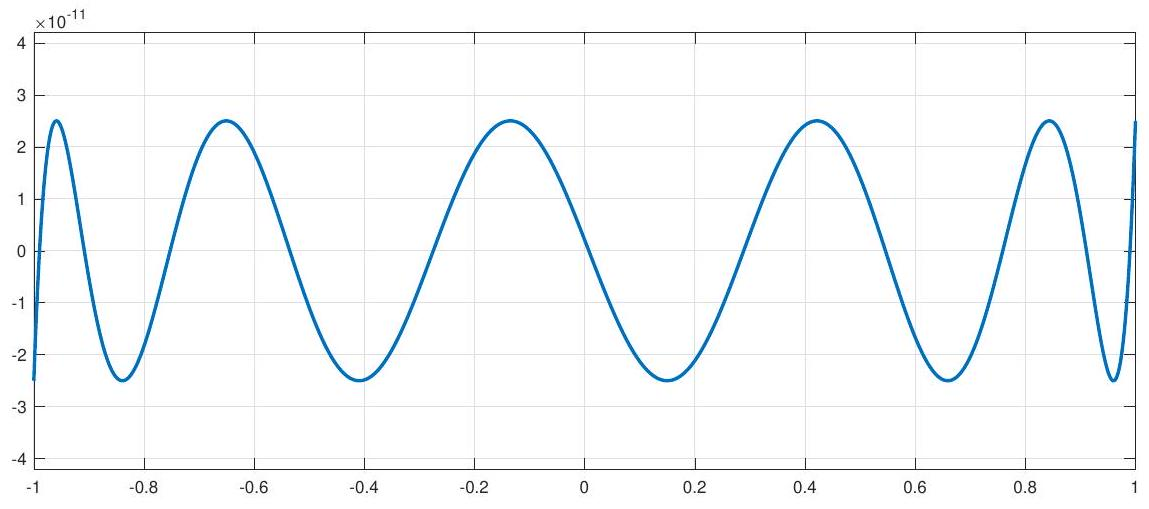
\includegraphics[width=12cm]{sheet 3 q 8}\end{center}
Make this precise by proving that equioscillation implies optimality: If $f-p_{k}$ has $k+2$ extrema $(a \leq)x_{1}<x_{2}<\cdots<x_{k+2}(\leq b)$ with alternating signs, i.e., $f\left(x_{i}\right)-p_{k}\left(x_{i}\right)=$ $(-1)^{i+\sigma}\left\|f-p_{k}\right\|_{\infty}$ where $\sigma=0$ or 1, then $p_{k}$ is a minimax polynomial approximant of degree $k$ to $f$. [\emph{Note: such computation can be done conveniently using Chebfun as e.g.} \verb|f = chebfun(@(x)exp(x)); p = minimax(f,10); plot(f-p)|\emph{. Note also that the equioscillation condition is in fact necessary and sufficient.}]



\question%9
\emph{Simpson's Rule} is a quadrature rule based on taking three sample points (endpoints $x_{0}, x_{2}$ and the center $x_{1}$), finding the quadratic polynomial interpolant, and integrating it.
\begin{parts}
\part%9a
Show that Simpson's rule applied to $I=\int_{x_{0}}^{x_{2}} f(x)~\mathrm d x$ gives the approximation $I \approx\frac{x_{1}-x_{0}}{3}[f(x_{0})+4 f(x_{1})+f(x_{2})]$.

\part%9b
Show further that Simpson's rule is exact if $f$ is a cubic polynomial.
\end{parts}



\question%10
(Optional:) Let $f$ be a polynomial of degree $2 n+1$, expressed as $f(x)=\sum_{i=0}^{2 n+1} c_{i} P_{i}(x)$, where $\{P_{i}(x)\}_{i=0}^{2 n+1}$ are orthonormal polynomials satisfying $\int_{-1}^{1} P_{i}(x) P_{j}(x)~\mathrm d x=\delta_{i j}$ (i.e., scaled Legendre polynomials).
\begin{parts}
\part%10a
Explain how to compute $c_{0}$ exactly by sampling $f$ at $n+1$ points.

\part%10b
Explain how to compute $c_{1}$ exactly by sampling $f$ at $n+2$ points.
\end{parts}

\end{questions}

\end{document}
